\section{A Temporal Kernel for Time Series}
\label{sec:kernel}

The method presented in this section consists in defining a kernel between
sets of timestamped objects (typically features).
This allows, in particular, to consider the case of irregularly sampled time
series.\footnote{This work was part of Adeline Bailly's PhD thesis.
We were co-supervising Adeline together with Laetitia Chapel.}

\subsection{Match kernel and Signature Quadratic Form Distance}

Our method relies on a user-chosen kernel $k(\cdot,\cdot)$ between local
features.
Based on this local kernel, one can compute the match kernel
\cite{NIPS2009_3874} between sets of local features as:

\begin{equation}
    K(\mathbf{x}, \mathbf{x}^\prime) = \sum_i \sum_j k(x_i, x^\prime_j).
\end{equation}

And the Signature Quadratic Form Distance (SQFD,
\cite{10.1145/1631272.1631391}) is the distance
between feature sets embedded in the Reproducing Kernel Hilbert Space (RKHS)
associated with $K$:

\begin{equation}
    SQFD(\mathbf{x}, \mathbf{x}^\prime) =
        \sqrt{K(\mathbf{x}, \mathbf{x})
              + K(\mathbf{x}^\prime, \mathbf{x}^\prime)
              - 2 K(\mathbf{x}, \mathbf{x}^\prime)}
        \, .
\end{equation}

\subsection{Local temporal kernel}

We introduce a time-sensitive local kernel defined as:

\begin{equation}
    k_t((x_i, t_i), (x^\prime_j, t^\prime_j)) = e^{\gamma_t (t^\prime_j - t_i)^2} k(x_i, x^\prime_j).
\end{equation}

This kernel is positive semi definite (psd), as the product of two psd kernels
and, if $k$ is the RBF kernel, it can be written as:

\begin{equation}
    k_t((x_i, t_i), (x^\prime_j, t^\prime_j)) = k(g(x_i, t_i), g(x^\prime_j, t^\prime_j)).
\end{equation}
with
\begin{equation}
g(x_i, t_i) = \left( x_{i,0}, \dots , x_{i, d-1},
                            \sqrt{\frac{\gamma_t}{\gamma_f}} t_i \right)
\end{equation}

Figure~\ref{fig:gamma_t} illustrates the impact of the ratio
$\sqrt{\frac{\gamma_t}{\gamma_f}}$ on the kernel matrix (larger $\gamma_t$
leads to ignoring off-diagonal elements).

\begin{figure}[t]
    \begin{subfigure}[b]{0.3\textwidth}
         \centering
         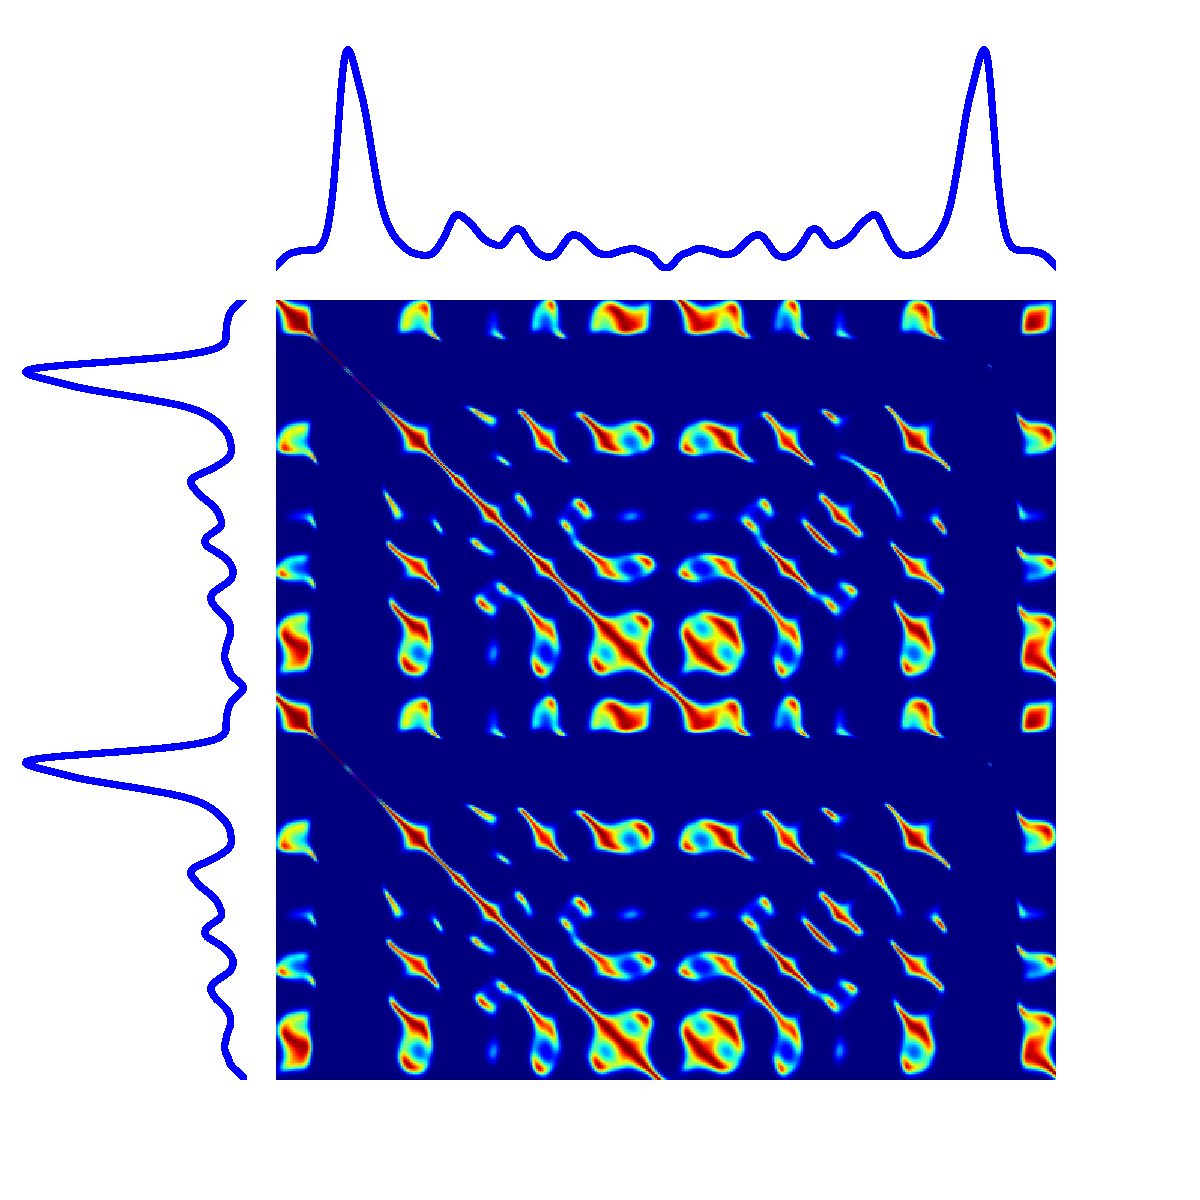
\includegraphics[width=\textwidth]{fig/gram_gammat0}
         \caption{$\gamma_t = 0$}
     \end{subfigure}
     \hfill
     \begin{subfigure}[b]{0.3\textwidth}
          \centering
          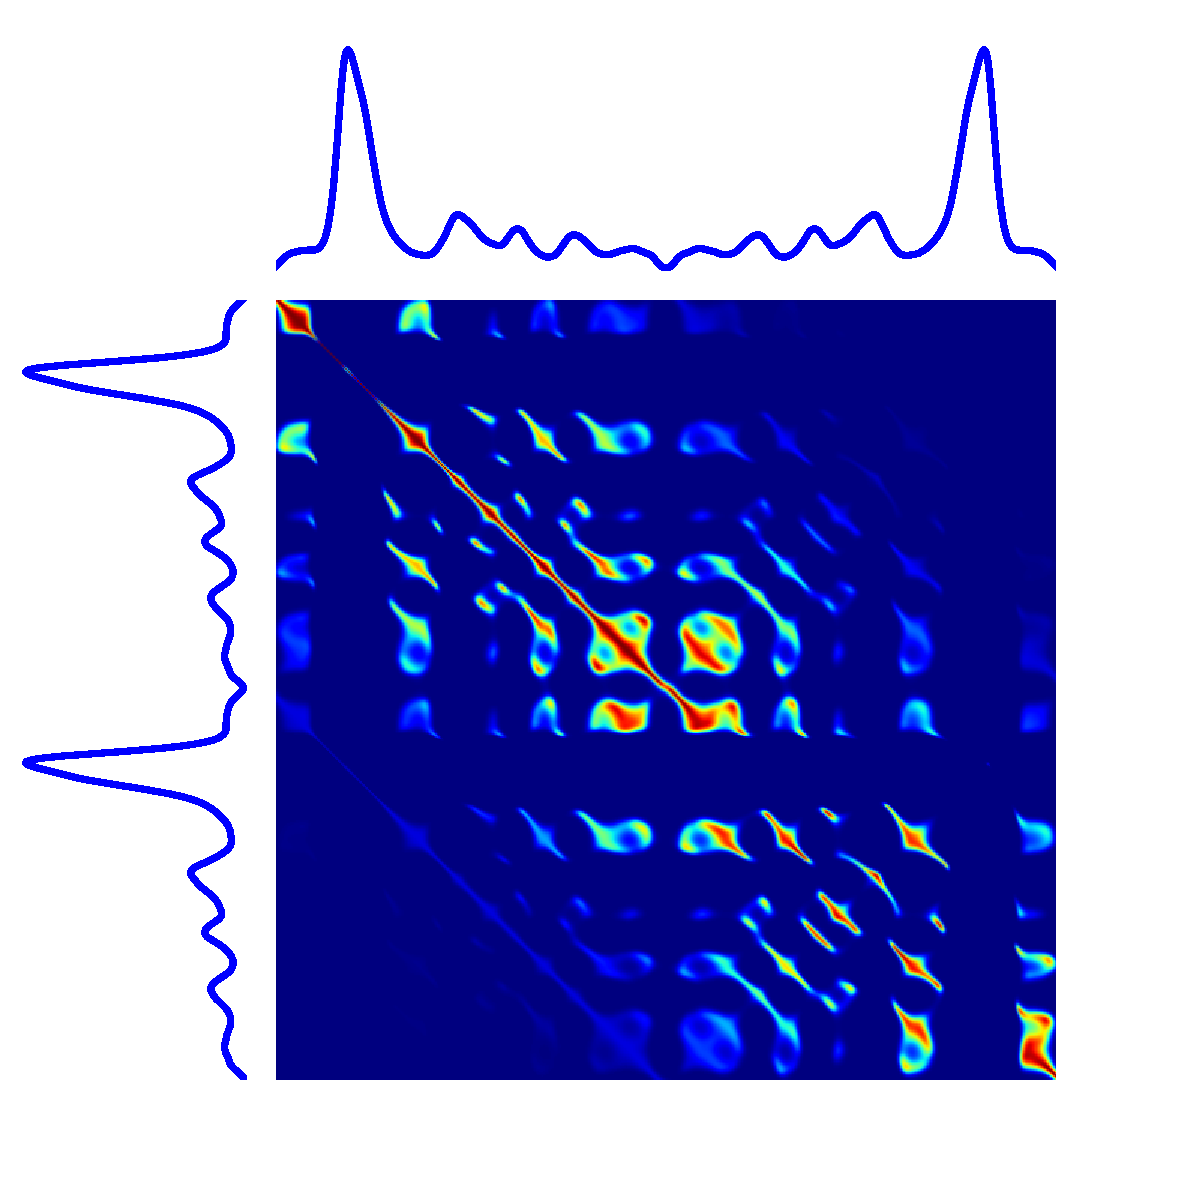
\includegraphics[width=\textwidth]{fig/gram_gammat10}
          \caption{Medium $\gamma_t$ value}
      \end{subfigure}
      \hfill
      \begin{subfigure}[b]{0.3\textwidth}
           \centering
           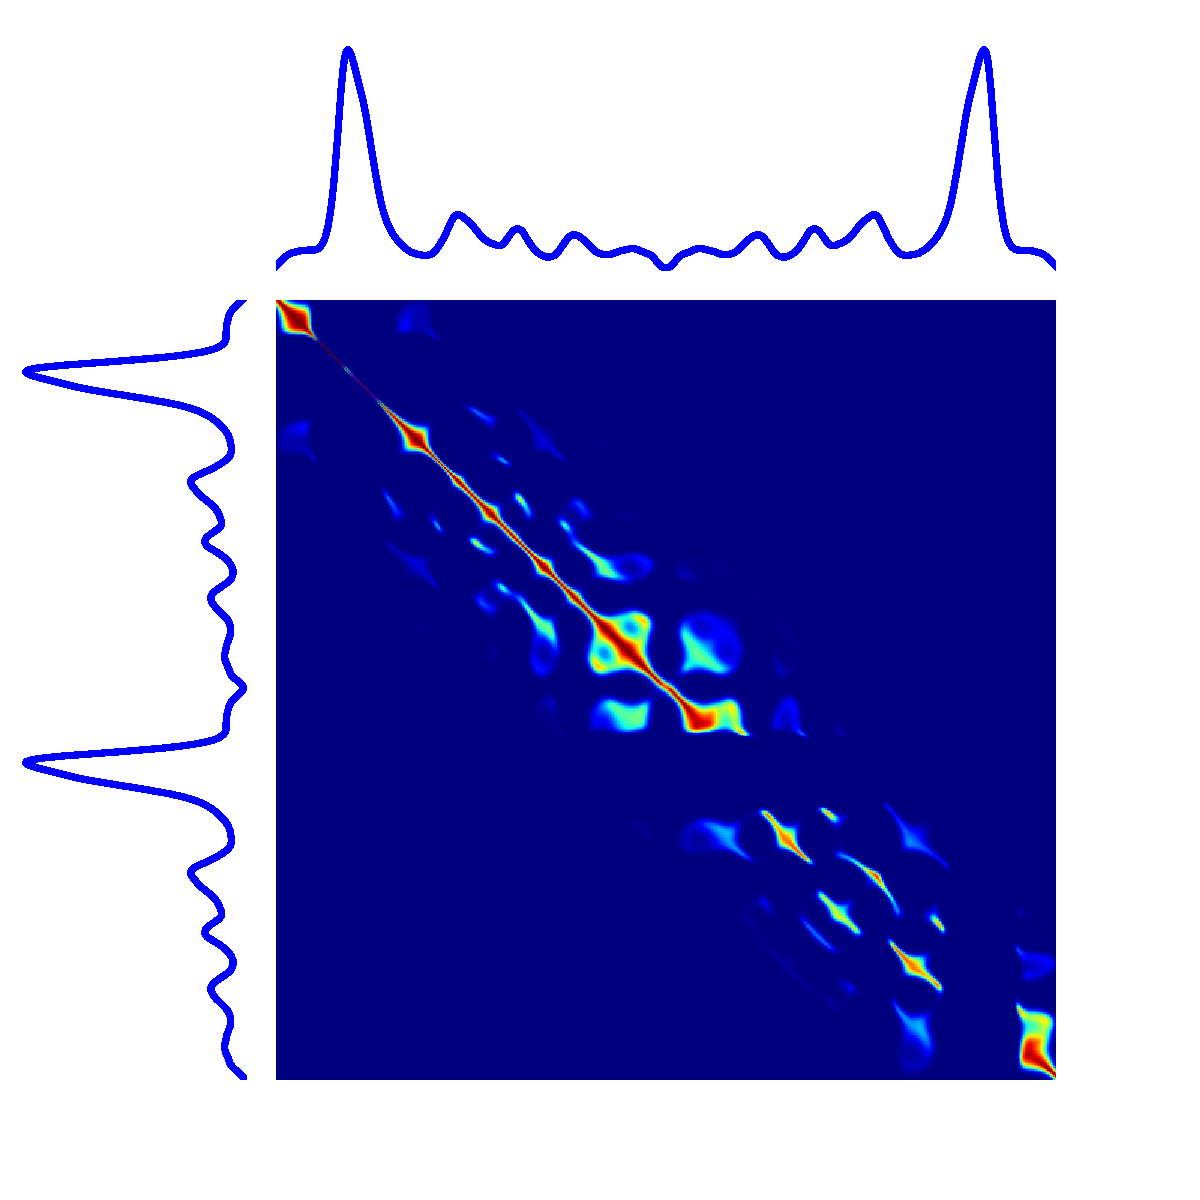
\includegraphics[width=\textwidth]{fig/gram_gammat100}
           \caption{Large $\gamma_t$ value}
       \end{subfigure}
    \caption{Impact of the $\gamma_t$ parameter on the kernel matrix on which
    SQFD relies.}
    \label{fig:gamma_t}
\end{figure}

$k_t$ is then a RBF kernel itself, and
Random Fourier Features \cite{NIPS2007_3182} can be
used in order to approximate it with a linear kernel.

Let us assume that we have a feature map $\phi$ such that

\begin{equation}
k_t((x_{i}, t_i), (x^\prime_j, t^\prime_j)) \approx
    \left\langle\phi(g(x_{i}, t_i)),
        \phi(g(x^\prime_{j}, t^\prime_j))\right\rangle,
\end{equation}
then we have:

\begin{equation}
SQFD(\mathbf{x}, \mathbf{x}^\prime) \approx \left\|
    \underbrace{\frac{1}{n}\sum_i \phi(g(x_{i}, t_i))}_{b_\phi(\mathbf{x})} -
    \underbrace{\frac{1}{m}\sum_j
        \phi(g(x^\prime_{j}, t^\prime_j))}_{b_\phi(\mathbf{x}^\prime)}
    \right\|.
\end{equation}

In other words, once feature sets are projected in this finite-dimensional
space, approximate SQFD computation is performed through (i) a barycenter
computation $b_\phi(\cdot)$ in the feature space (which can be done offline)
followed by (ii) a Euclidean distance computation in $O(D)$ time, where $D$ is
the dimension of the feature map $\phi(x)$.
Overall, we have a distance between timestamped feature sets whose
precision / complexity tradeoff can be tuned via the map dimensionality $D$.

\subsection{Evaluation}

In order to evaluate the method presented above, we have used the UCR Time
Series Classification archive, which, at the time, was made of monodimensional
time series only.
We decided not to work on raw data but rather extract local features to
describe our time series.
We chose to rely on temporal SIFT features, that we had introduced in
\cite{bailly:halshs-01184900,bailly:hal-01252726}.
These features are straight-forward 1D adaptations of the Scale-Invariant
Feature Transform (SIFT) framework introduced in Computer Vision
\cite{Lowe:2004:DIF:993451.996342}.%
\footnote{Note that the use of such handcrafted features was already outdated in the
computer vision community at the time of this work.
However, in our small data context, they proved useful for the task at hand.}

We show in \cite{tavenard:halshs-01561461} that kernel approximation
leads to better trade-offs in terms of computational
complexity \emph{vs.} kernel approximation than a pre-processing of the feature sets
that would rely on $k$-means clustering.
We also show that the obtained distance, once embedded in a Support Vector
Machine with Gaussian kernel, leads to classification performance that is
competitive with the state-of-the-art.
